\documentclass[12pt,a4paper]{article}
\usepackage[utf8]{inputenc}
\usepackage[spanish]{babel}
\usepackage{amsmath}
\usepackage{amsfonts}
\usepackage{amssymb}
\usepackage{graphicx}
\usepackage{array,tabularx}
\usepackage[left=2cm,right=2cm,top=2cm,bottom=2cm]{geometry}
\begin{document}
\begin{titlepage}
	\begin{center}
	{\huge \textbf{Universidad Veracruzana}}\\
	\vspace{2cm}  
	{\Large {Documento de descripcion}}\\
	\vspace{5mm}	
	{\Large {Google Fotoss}}\\
	\begin{figure}[h]
		\centering
		
\includegraphics[scale=0.10]{uvlogo}
	\end{figure}
	{\Large {Ingeniería de software}}\\
    \vspace{2cm}
	{\Large {García Sosa Oswaldo }}\\
	\vspace{25mm}	
    \rule{8cm}{0.5mm} \\ \Large Vo.bo\\ 
	\end{center}
\end{titlepage}
\vspace{1 cm}
\section{Introduccion}
	La pagina google fotos fue creada con react y firebase como medio de almacenamiento, tambien cuenta con un registro de usuario mediante facebook, todo para una mayor comodidad para poder iniciar a la pagina. Google Fotos se basa en un sistema de guardado y gestion de albums, por lo cual primero se debera nombrar un album, para poder seleccionarlo y subir imagenes que deseas que lo integren.\\

\section{Login}
	Lo primero que se vera al iniciar en la pagina sera un boton con acceso a logearse por medio de Facebook, todo esto haciendo que sea facil para cualquier usuario. Ya que hoy en dia la mayoria de las personas tienen una cuenta con este servicio.\\

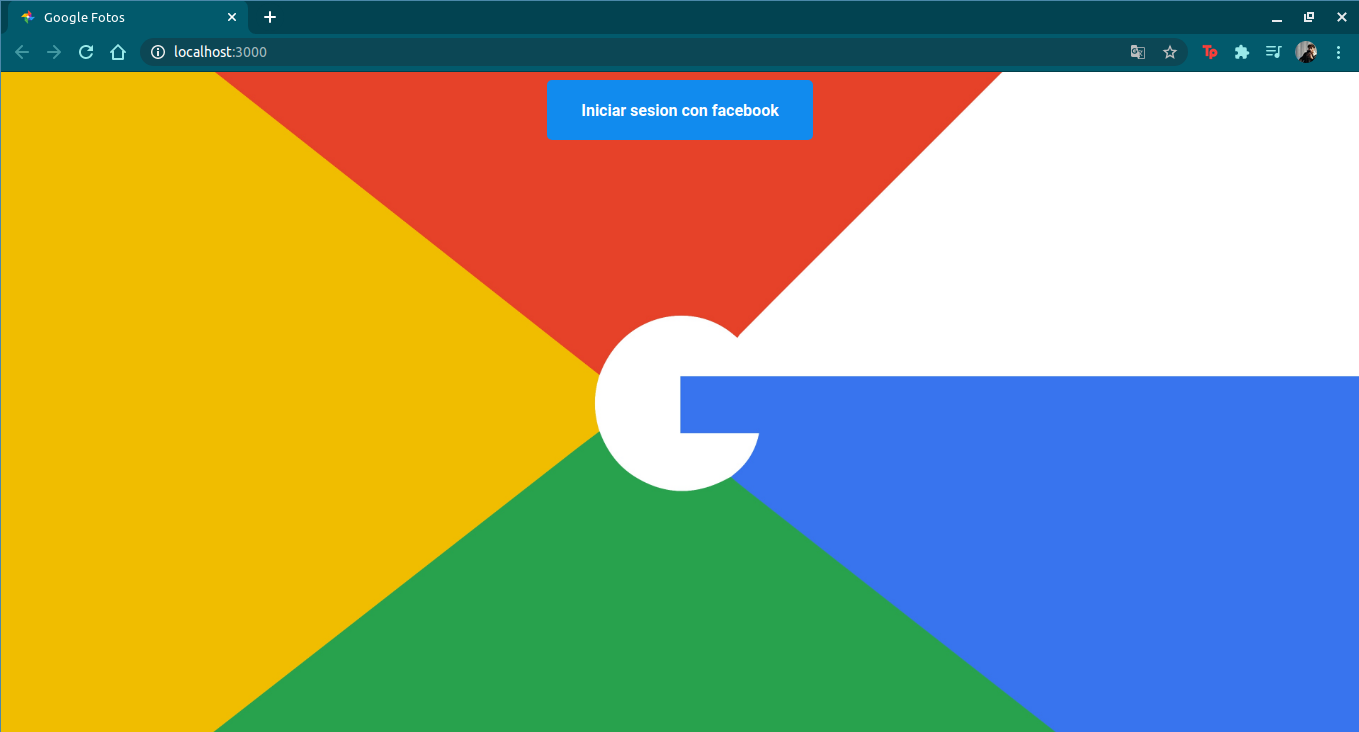
\includegraphics[scale=0.20]{Login}

\section{Inicio}
	Al acceder con una cuenta de facebook, en el inicio de la pagina podremos ver en la parte de arriba un navbar para poder regresar al inicio presionando el nombre de la pagina, ademas a eso se tiene un boton para cerrar sesion y informacion acerca del usuario ingresado, su informacion sera su nombre y su foto de perfil. En la parte de abajo se encontraran todos los albums creados por el usuario, estos albums contaran con una foto de portada y su nombre. Finalmente en la parte de abajo contaremos con la opcion de poder crear los albums.\\

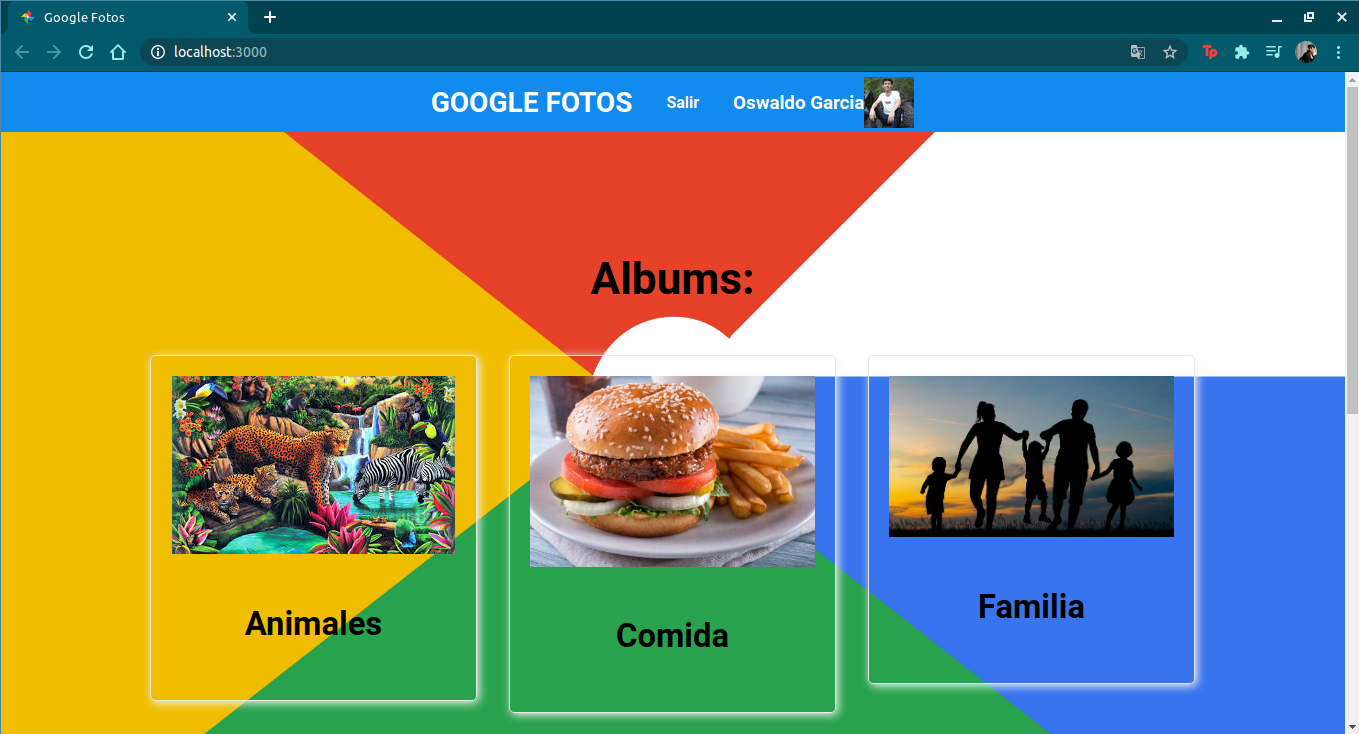
\includegraphics[scale=0.20]{Inicio1}

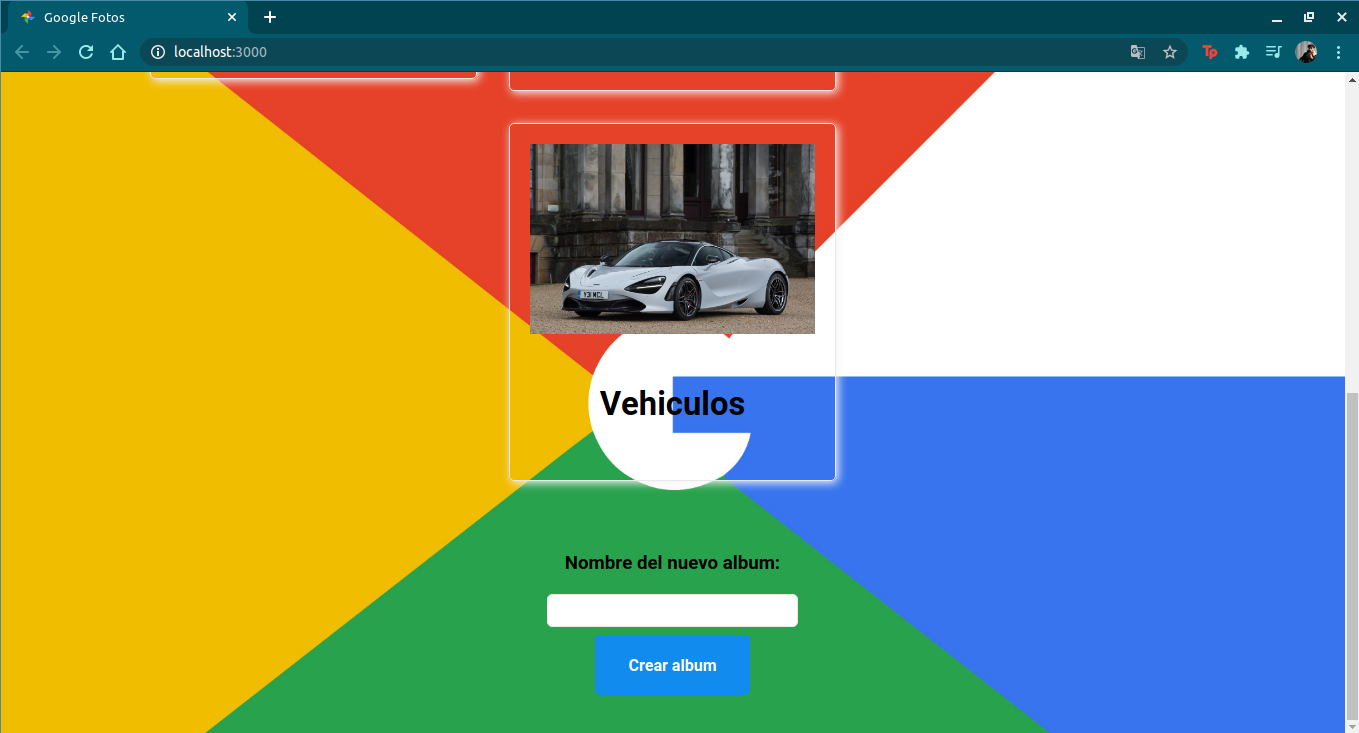
\includegraphics[scale=0.20]{Inicio2}

\section{Album}
	Una vez creado un album se puede acceder a el con un simple click, una vez ahi simplemente se debera agregar las fotos que deseas tener en ese album, considerando que se debe subir una por una.

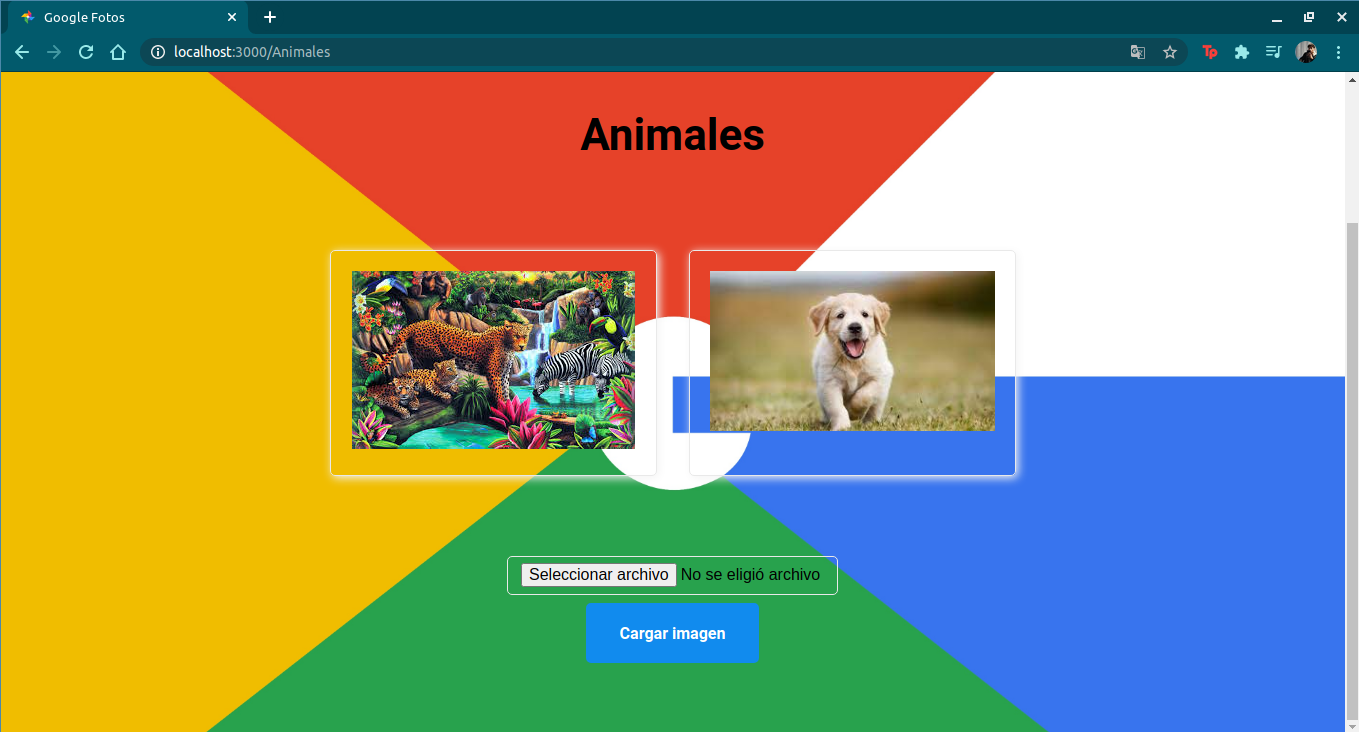
\includegraphics[scale=0.20]{Album}

\end{document}
